\documentclass[11pt,a4paper,twoside]{article}

\usepackage[T1]{fontenc}
\usepackage[utf8]{inputenc}
\usepackage{lmodern}
\usepackage{amsmath,amssymb,mathtools}
\usepackage{geometry}
\usepackage{array,booktabs,multirow,tabularx}
\usepackage{enumitem}
\usepackage{xcolor}
\usepackage{tikz}
\usepackage{eso-pic}
\usepackage{hyperref}
\usetikzlibrary{positioning,arrows.meta,shapes.geometric,calc,fit}

\geometry{margin=0.85in,headheight=15pt,headsep=18pt,footskip=24pt}
\setlength{\parindent}{0pt}
\setlength{\parskip}{5pt}
\setlist[itemize]{leftmargin=1.7em,itemsep=2pt,topsep=3pt}
\setlist[enumerate]{leftmargin=1.9em,itemsep=2pt,topsep=3pt}

\definecolor{navy}{HTML}{163A5F}
\definecolor{blue}{HTML}{2E74B5}
\definecolor{lightblue}{HTML}{EAF3FA}
\definecolor{lightgreen}{HTML}{EAF6EF}
\definecolor{lightorange}{HTML}{FFF3E4}
\definecolor{lightgray}{HTML}{F2F4F7}
\definecolor{darkgray}{HTML}{4A5568}

\hypersetup{
  colorlinks=true,
  linkcolor=navy,
  urlcolor=blue,
  pdftitle={RNNs, Seq2Seq, Attention, and Transformers: Mathematical Notes},
  pdfauthor={Md. Atikuzzaman}
}

\pagestyle{empty}
\AddToShipoutPictureFG{%
  \AtPageUpperLeft{%
    \raisebox{-0.47in}[0pt][0pt]{%
      \hspace*{0.85in}%
      \makebox[\dimexpr\paperwidth-1.70in\relax][l]{%
        \small RNNs, Seq2Seq, Attention, and Transformers\hfill Mathematical Notes}}}%
  \AtPageUpperLeft{%
    \raisebox{-0.60in}[0pt][0pt]{%
      \hspace*{0.85in}\rule{\dimexpr\paperwidth-1.70in\relax}{0.4pt}}}%
  \AtPageLowerLeft{%
    \raisebox{0.70in}[0pt][0pt]{%
      \hspace*{0.85in}\rule{\dimexpr\paperwidth-1.70in\relax}{0.4pt}}}%
  \AtPageLowerLeft{%
    \raisebox{0.53in}[0pt][0pt]{%
      \hspace*{0.85in}%
      \makebox[\dimexpr\paperwidth-1.70in\relax][l]{%
        \small Prepared By: Md. Atikuzzaman\hfill Page \thepage}}}%
}

\newcommand{\R}{\mathbb{R}}
\newcommand{\E}{\mathbb{E}}
\newcommand{\norm}[1]{\left\lVert#1\right\rVert}
\newcommand{\softmax}{\operatorname{softmax}}
\newcommand{\sigmoid}{\operatorname{sigmoid}}
\newcommand{\keybox}[2]{%
  \begin{center}
  \begin{tikzpicture}
    \node[draw=blue!55,fill=#1,rounded corners=2pt,
      inner sep=8pt,text width=0.92\textwidth,align=left] {#2};
  \end{tikzpicture}
  \end{center}
}

\begin{document}

\begin{center}
  {\color{navy}\bfseries\LARGE RNNs, Sequence-to-Sequence Learning,}\\[2pt]
  {\color{navy}\bfseries\LARGE Attention Mechanism, and Transformers}\\[4pt]
  {\color{blue}\bfseries\Large Mathematical Notes}\\[10pt]
  {\small Recurrent States, BPTT, LSTM, GRU, Encoder-Decoder Learning, Teacher Forcing, Attention, Q-K-V, Self-Attention, Multi-Head Attention, Positional Encoding, and Applications}
\end{center}

\keybox{lightblue}{\textbf{Central idea.} Sequence models learn from ordered observations. RNNs carry information through recurrent states, gated models control memory, Seq2Seq models map one sequence to another, attention selects relevant states dynamically, and Transformers replace recurrence with parallel attention-based interactions.}

\subsection*{Concept Map}

\begin{center}
\resizebox{0.98\textwidth}{!}{%
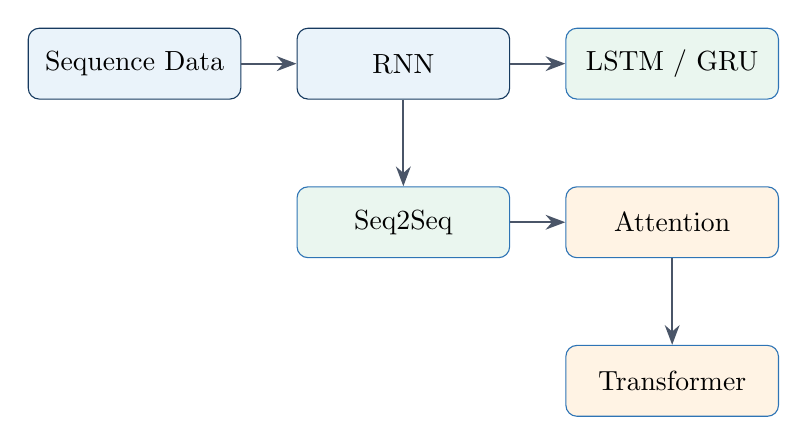
\begin{tikzpicture}[
  box/.style={draw=navy,rounded corners,minimum width=2.7cm,minimum height=0.9cm,align=center,fill=lightblue},
  gate/.style={draw=blue,rounded corners,minimum width=2.7cm,minimum height=0.9cm,align=center,fill=lightgreen},
  trans/.style={draw=blue,rounded corners,minimum width=2.7cm,minimum height=0.9cm,align=center,fill=lightorange},
  arr/.style={-{Stealth[length=2.5mm]},thick,color=darkgray}
]
  \node[box] (seq) {Sequence Data};
  \node[box,right=0.7cm of seq] (rnn) {RNN};
  \node[gate,right=0.7cm of rnn] (gates) {LSTM / GRU};
  \node[gate,below=1.1cm of rnn] (s2s) {Seq2Seq};
  \node[trans,right=0.7cm of s2s] (att) {Attention};
  \node[trans,below=1.1cm of att] (tr) {Transformer};
  \draw[arr] (seq)--(rnn);
  \draw[arr] (rnn)--(gates);
  \draw[arr] (rnn)--(s2s);
  \draw[arr] (s2s)--(att);
  \draw[arr] (att)--(tr);
\end{tikzpicture}}
\end{center}

% ============================================================
\section*{I. Sequence Data and Recurrent Neural Networks}
% ============================================================

\subsection*{1. Why Sequence Models?}

A sequence is an ordered collection

\[
X=(x_1,x_2,\ldots,x_T).
\]

The order often carries essential information. Examples include sentences, speech, sensor measurements, financial time series, weather observations, and user-click histories.

\textbf{Worked example: order changes meaning.}

Consider two token sequences:

\[
S_1=(\text{dog},\text{bites},\text{man}),
\]

\[
S_2=(\text{man},\text{bites},\text{dog}).
\]

Both have the same unigram count vector over

\[
V=\{\text{dog},\text{bites},\text{man}\}:
\]

\[
x_{S_1}=x_{S_2}=(1,1,1).
\]

However, their bigram sets differ:

\[
B(S_1)=\{\text{dog bites},\text{bites man}\},
\]

\[
B(S_2)=\{\text{man bites},\text{bites dog}\}.
\]

Thus a representation that ignores order cannot distinguish these meanings.

\subsection*{2. Basic RNN State Update}

An RNN updates its hidden state using

\[
\boxed{h_t=\tanh(W_{xh}x_t+W_{hh}h_{t-1}+b_h)}.
\]

The output may be computed by

\[
\boxed{\hat y_t=g(W_{hy}h_t+b_y)},
\]

where $g$ is selected for the task, such as sigmoid for binary prediction or softmax for multiclass prediction.

The same parameters are reused at every time step.

\begin{center}
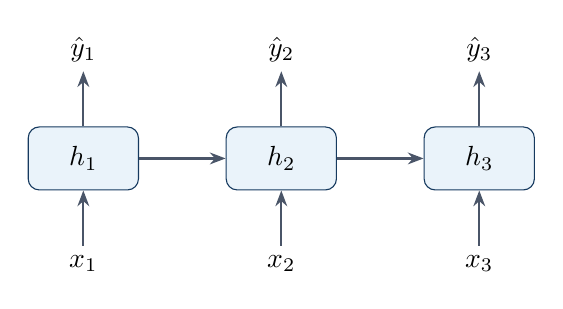
\begin{tikzpicture}[
  cell/.style={draw=navy,rounded corners,fill=lightblue,minimum width=1.4cm,minimum height=0.8cm,align=center},
  arr/.style={-{Stealth[length=2mm]},thick,color=darkgray}
]
  \node[cell] (h1) {$h_1$};
  \node[cell,right=1.1cm of h1] (h2) {$h_2$};
  \node[cell,right=1.1cm of h2] (h3) {$h_3$};
  \node[below=0.7cm of h1] (x1) {$x_1$};
  \node[below=0.7cm of h2] (x2) {$x_2$};
  \node[below=0.7cm of h3] (x3) {$x_3$};
  \node[above=0.7cm of h1] (y1) {$\hat y_1$};
  \node[above=0.7cm of h2] (y2) {$\hat y_2$};
  \node[above=0.7cm of h3] (y3) {$\hat y_3$};
  \draw[arr] (x1)--(h1); \draw[arr] (x2)--(h2); \draw[arr] (x3)--(h3);
  \draw[arr] (h1)--(h2); \draw[arr] (h2)--(h3);
  \draw[arr] (h1)--(y1); \draw[arr] (h2)--(y2); \draw[arr] (h3)--(y3);
\end{tikzpicture}
\end{center}

\textbf{Worked example: scalar RNN forward pass.}

Let

\[
W_{xh}=0.5,\quad W_{hh}=0.8,\quad b_h=0,\quad h_0=0,
\]

and

\[
(x_1,x_2,x_3)=(1,2,-1).
\]

At $t=1$,

\[
a_1=0.5(1)+0.8(0)=0.5,
\]

\[
h_1=\tanh(0.5)=0.4621.
\]

At $t=2$,

\[
a_2=0.5(2)+0.8(0.4621)=1.3697,
\]

\[
h_2=\tanh(1.3697)=0.8786.
\]

At $t=3$,

\[
a_3=0.5(-1)+0.8(0.8786)=0.2029,
\]

\[
h_3=\tanh(0.2029)=0.2002.
\]

\begin{center}
\begin{tabular}{c|c|c|c}
\toprule
$t$&$x_t$&Preactivation $a_t$&Hidden state $h_t$\\ \midrule
1&1&0.5000&0.4621\\
2&2&1.3697&0.8786\\
3&$-1$&0.2029&0.2002\\ \bottomrule
\end{tabular}
\end{center}

Let $W_{hy}=1.2$ and $b_y=-0.1$. A final binary output is

\[
\hat y_3=\sigmoid(1.2h_3-0.1)
=\sigmoid(0.1402)
\approx0.5350.
\]

\[
\boxed{h_3\approx0.2002,\qquad\hat y_3\approx0.5350.}
\]

\subsection*{3. RNN Input-Output Structures}

\begin{center}
\begin{tabularx}{0.97\textwidth}{>{\bfseries}p{3.3cm}XX}
\toprule
Structure&Example&Mapping\\ \midrule
One-to-one&Image classification&one input to one output\\
One-to-many&Image captioning&one input to an output sequence\\
Many-to-one&Sentiment classification&input sequence to one label\\
Many-to-many aligned&POS tagging&one output per input position\\
Many-to-many unaligned&Translation&input and output lengths differ\\ \bottomrule
\end{tabularx}
\end{center}

\textbf{Worked example: output-shape calculation.}

Suppose a batch contains $B=32$ sequences, each with $T=20$ positions. The hidden dimension is $d_h=64$ and the tag set has $d_y=10$ classes.

For aligned many-to-many tagging,

\[
H\in\R^{32\times20\times64},
\]

and the output logits have shape

\[
Y\in\R^{32\times20\times10}.
\]

The number of output logits is

\[
32\times20\times10=6400.
\]

For many-to-one classification, only the final state is used, so the output shape becomes

\[
Y_{\mathrm{many\text{-}to\text{-}one}}\in\R^{32\times10},
\]

containing

\[
32\times10=320
\]

logits.

\subsection*{4. RNN Parameter Count}

For input dimension $d_x$, hidden dimension $d_h$, and output dimension $d_y$, a basic RNN has

\[
W_{xh}\in\R^{d_h\times d_x},\quad
W_{hh}\in\R^{d_h\times d_h},\quad
b_h\in\R^{d_h},
\]

\[
W_{hy}\in\R^{d_y\times d_h},\quad
b_y\in\R^{d_y}.
\]

Therefore,

\[
\boxed{P=d_hd_x+d_h^2+d_h+d_yd_h+d_y.}
\]

\textbf{Worked example: parameter counting.}

Let $d_x=3$, $d_h=4$, and $d_y=2$.

\begin{center}
\begin{tabular}{c|c|c}
\toprule
Parameter&Shape&Count\\ \midrule
$W_{xh}$&$4\times3$&12\\
$W_{hh}$&$4\times4$&16\\
$b_h$&$4$&4\\
$W_{hy}$&$2\times4$&8\\
$b_y$&$2$&2\\ \midrule
Total&&42\\ \bottomrule
\end{tabular}
\end{center}

\[
\boxed{P=12+16+4+8+2=42.}
\]

This count does not grow with sequence length because the parameters are shared across time.

% ============================================================
\section*{II. Backpropagation Through Time}
% ============================================================

An unrolled RNN is trained by Backpropagation Through Time (BPTT). A gradient reaching an earlier state contains a product of recurrent Jacobians:

\[
\boxed{
\frac{\partial L}{\partial h_k}
=
\frac{\partial L}{\partial h_t}
\prod_{j=k+1}^{t}
\frac{\partial h_j}{\partial h_{j-1}}
}.
\]

Repeated multiplication can cause vanishing or exploding gradients.

\subsection*{1. Vanishing and Exploding Gradients}

\textbf{Worked example: repeated gradient factors.}

Assume the magnitude of the local recurrent derivative is constant.

For a derivative factor $0.5$ across ten steps,

\[
g_{\mathrm{early}}=(0.5)^{10}=0.0009766.
\]

The gradient becomes almost zero.

For a derivative factor $1.5$ across ten steps,

\[
g_{\mathrm{early}}=(1.5)^{10}=57.665.
\]

The gradient becomes very large.

\begin{center}
\begin{tabular}{c|c|c}
\toprule
Local factor&Ten-step product&Effect\\ \midrule
$0.5$&$0.0009766$&Vanishing\\
$1.0$&$1.0000$&Stable magnitude\\
$1.5$&$57.665$&Exploding\\ \bottomrule
\end{tabular}
\end{center}

\subsection*{2. Gradient Clipping}

If the gradient norm exceeds threshold $\tau$, norm clipping uses

\[
\boxed{
g_{\mathrm{clip}}=g\frac{\tau}{\norm{g}_2}
\quad\text{when }\norm{g}_2>\tau.
}
\]

\textbf{Worked example: clipping an exploding gradient.}

Let

\[
g=\begin{bmatrix}6\\8\end{bmatrix},
\qquad
\norm{g}_2=\sqrt{6^2+8^2}=10,
\]

and let $\tau=5$. Then

\[
g_{\mathrm{clip}}
=\begin{bmatrix}6\\8\end{bmatrix}\frac5{10}
=\begin{bmatrix}3\\4\end{bmatrix}.
\]

The clipped norm is

\[
\norm{g_{\mathrm{clip}}}_2=\sqrt{3^2+4^2}=5.
\]

\[
\boxed{g_{\mathrm{clip}}=(3,4)^\top.}
\]

% ============================================================
\section*{III. Gated Recurrent Networks}
% ============================================================

\subsection*{1. Long Short-Term Memory}

An LSTM introduces a persistent cell state $c_t$ and gates that control information flow:

\[
f_t=\sigmoid(W_f[h_{t-1},x_t]+b_f),
\]

\[
i_t=\sigmoid(W_i[h_{t-1},x_t]+b_i),
\]

\[
\tilde c_t=\tanh(W_c[h_{t-1},x_t]+b_c),
\]

\[
o_t=\sigmoid(W_o[h_{t-1},x_t]+b_o),
\]

\[
\boxed{c_t=f_t\odot c_{t-1}+i_t\odot\tilde c_t},
\]

\[
\boxed{h_t=o_t\odot\tanh(c_t)}.
\]

\textbf{Worked example: one scalar LSTM step.}

Suppose

\[
h_{t-1}=0.2,
\qquad
c_{t-1}=0.4,
\qquad
x_t=0.7,
\]

and the learned gate preactivations are

\[
a_f=1.0,
\quad a_i=0.2,
\quad a_c=0.5,
\quad a_o=0.8.
\]

Then

\[
f_t=\sigmoid(1.0)=0.7311,
\]

\[
i_t=\sigmoid(0.2)=0.5498,
\]

\[
\tilde c_t=\tanh(0.5)=0.4621,
\]

\[
o_t=\sigmoid(0.8)=0.6900.
\]

The new cell state is

\[
\begin{aligned}
c_t
&=0.7311(0.4)+0.5498(0.4621)\\
&=0.2924+0.2541\\
&=0.5465.
\end{aligned}
\]

The new hidden state is

\[
h_t=0.6900\tanh(0.5465)
\approx0.6900(0.4979)
\approx0.3436.
\]

\begin{center}
\begin{tabular}{c|c|c}
\toprule
Quantity&Activation&Value\\ \midrule
Forget gate&$\sigmoid(1.0)$&$0.7311$\\
Input gate&$\sigmoid(0.2)$&$0.5498$\\
Candidate&$\tanh(0.5)$&$0.4621$\\
Output gate&$\sigmoid(0.8)$&$0.6900$\\
Cell state&&$0.5465$\\
Hidden state&&$0.3436$\\ \bottomrule
\end{tabular}
\end{center}

\[
\boxed{c_t\approx0.5465,\qquad h_t\approx0.3436.}
\]

\subsection*{2. Gated Recurrent Unit}

A GRU uses update and reset gates:

\[
z_t=\sigmoid(W_z[h_{t-1},x_t]),
\]

\[
r_t=\sigmoid(W_r[h_{t-1},x_t]),
\]

\[
\tilde h_t=\tanh(W_h[r_t\odot h_{t-1},x_t]),
\]

\[
\boxed{h_t=(1-z_t)\odot h_{t-1}+z_t\odot\tilde h_t}.
\]

\textbf{Worked example: one scalar GRU step.}

Let

\[
h_{t-1}=0.4,
\quad x_t=0.6,
\quad z_t=0.6,
\quad r_t=0.25.
\]

Assume the candidate calculation is

\[
\tilde h_t=\tanh\left(0.8(r_th_{t-1})+0.5x_t\right).
\]

First,

\[
r_th_{t-1}=0.25(0.4)=0.1.
\]

Thus,

\[
\tilde h_t
=\tanh(0.8(0.1)+0.5(0.6))
=\tanh(0.38)
\approx0.3627.
\]

The state update is

\[
\begin{aligned}
h_t
&=(1-0.6)(0.4)+0.6(0.3627)\\
&=0.16+0.2176\\
&=0.3776.
\end{aligned}
\]

\[
\boxed{h_t\approx0.3776.}
\]

\subsection*{3. Parameter Comparison}

Ignoring output layers, with input size $d_x$ and hidden size $d_h$:

\[
P_{\mathrm{RNN}}=d_hd_x+d_h^2+d_h,
\]

\[
P_{\mathrm{GRU}}=3P_{\mathrm{RNN}},
\]

\[
P_{\mathrm{LSTM}}=4P_{\mathrm{RNN}}.
\]

\textbf{Worked example: gated-model parameter count.}

Let $d_x=10$ and $d_h=20$. Then

\[
P_{\mathrm{RNN}}=20(10)+20^2+20=620,
\]

\[
P_{\mathrm{GRU}}=3(620)=1860,
\]

\[
P_{\mathrm{LSTM}}=4(620)=2480.
\]

\begin{center}
\begin{tabular}{c|c|c}
\toprule
Model&Number of gate/state transformations&Parameters\\ \midrule
Simple RNN&1&620\\
GRU&3&1860\\
LSTM&4&2480\\ \bottomrule
\end{tabular}
\end{center}

The additional parameters give gated models greater control over memory.

% ============================================================
\section*{IV. Sequence-to-Sequence Learning}
% ============================================================

Seq2Seq maps a source sequence

\[
x=(x_1,\ldots,x_{T_x})
\]

to a target sequence

\[
y=(y_1,\ldots,y_{T_y}),
\]

where $T_x$ and $T_y$ may differ.

\begin{center}
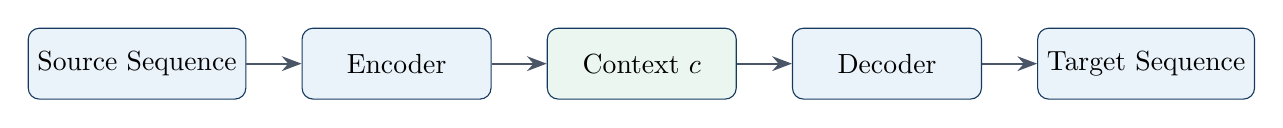
\begin{tikzpicture}[
  box/.style={draw=navy,rounded corners,fill=lightblue,minimum width=2.4cm,minimum height=0.9cm,align=center},
  arr/.style={-{Stealth[length=2.5mm]},thick,color=darkgray}
]
  \node[box] (src) {Source Sequence};
  \node[box,right=0.7cm of src] (enc) {Encoder};
  \node[box,right=0.7cm of enc,fill=lightgreen] (ctx) {Context $c$};
  \node[box,right=0.7cm of ctx] (dec) {Decoder};
  \node[box,right=0.7cm of dec] (tgt) {Target Sequence};
  \draw[arr] (src)--(enc); \draw[arr] (enc)--(ctx); \draw[arr] (ctx)--(dec); \draw[arr] (dec)--(tgt);
\end{tikzpicture}
\end{center}

\subsection*{1. Encoder and Fixed Context Vector}

The encoder computes

\[
h_t^{\mathrm{enc}}=f_{\mathrm{enc}}(x_t,h_{t-1}^{\mathrm{enc}}),
\]

and a basic Seq2Seq model uses

\[
\boxed{c=h_{T_x}^{\mathrm{enc}}}
\]

as a fixed context vector.

\textbf{Worked example: scalar encoder.}

Let

\[
h_t=\tanh(0.7x_t+0.6h_{t-1}),
\qquad h_0=0,
\]

and

\[
(x_1,x_2,x_3)=(1,0.5,-0.5).
\]

Then

\[
h_1=\tanh(0.7)=0.6044,
\]

\[
h_2=\tanh(0.7(0.5)+0.6(0.6044))
=\tanh(0.7126)
=0.6123,
\]

\[
h_3=\tanh(0.7(-0.5)+0.6(0.6123))
=\tanh(0.0174)
=0.0174.
\]

Therefore,

\[
\boxed{c=h_3=0.0174.}
\]

The final scalar must summarize the complete three-token source, illustrating the fixed-vector bottleneck.

\subsection*{2. Conditional Sequence Probability and Loss}

The decoder factorizes the target probability as

\[
\boxed{
P(y\mid x)=\prod_{t=1}^{T_y}P(y_t\mid y_{<t},c)
}.
\]

The sequence negative log-likelihood is

\[
\boxed{
L=-\sum_{t=1}^{T_y}\log P(y_t\mid y_{<t},c)
}.
\]

\textbf{Worked example: target-sequence probability.}

Suppose the correct target has three tokens with conditional probabilities

\begin{center}
\begin{tabular}{c|c|c}
\toprule
Step&Correct token&Conditional probability\\ \midrule
1&$y_1$&$0.80$\\
2&$y_2$&$0.70$\\
3&$\langle\mathrm{EOS}\rangle$&$0.90$\\ \bottomrule
\end{tabular}
\end{center}

Then

\[
P(y\mid x)=0.80(0.70)(0.90)=0.504.
\]

The loss is

\[
L=-\log(0.504)\approx0.685.
\]

The average token loss is

\[
\bar L=\frac{0.685}{3}\approx0.228.
\]

\[
\boxed{P(y\mid x)=0.504,\qquad L\approx0.685.}
\]

\subsection*{3. Teacher Forcing}

During training, teacher forcing uses the correct previous token rather than the model's previous prediction:

\[
y_{t-1}^{\mathrm{true}}\rightarrow\text{Decoder}\rightarrow\hat y_t.
\]

\textbf{Worked example: expected number of teacher-forced steps.}

Suppose a target contains $T_y=20$ decoding steps and teacher forcing is applied independently with probability $p_{TF}=0.75$.

The expected number of teacher-forced steps is

\[
\E[N_{TF}]=T_yp_{TF}=20(0.75)=15.
\]

The expected number of steps using model predictions is

\[
20-15=5.
\]

\[
\boxed{\E[N_{TF}]=15,\qquad\E[N_{\mathrm{model}}]=5.}
\]

Teacher forcing stabilizes training, but the difference between training and inference creates exposure bias.

\subsection*{4. Greedy and Beam-Search Decoding}

Greedy decoding chooses the highest-probability token at each step. Beam search retains several partial sequences.

\textbf{Worked example: greedy versus beam search.}

At the first step,

\[
P(A)=0.55,
\qquad
P(B)=0.45.
\]

If $A$ is chosen, the next probability of $\langle\mathrm{EOS}\rangle$ is $0.50$:

\[
P(A,\mathrm{EOS})=0.55(0.50)=0.275.
\]

If $B$ is retained by a beam, the next token $C$ has probability $0.90$ and then EOS has probability $0.80$:

\[
P(B,C,\mathrm{EOS})=0.45(0.90)(0.80)=0.324.
\]

Although greedy decoding initially prefers $A$,

\[
0.324>0.275.
\]

Therefore, a beam can recover the higher-probability complete sequence

\[
\boxed{B\rightarrow C\rightarrow\mathrm{EOS}.}
\]

% ============================================================
\section*{V. Attention Mechanism}
% ============================================================

Attention removes the need to compress all source information into one fixed context vector. At decoder step $t$,

\[
e_{t,i}=\operatorname{Score}(h_{t-1}^{\mathrm{dec}},h_i^{\mathrm{enc}}),
\]

\[
\boxed{
\alpha_{t,i}=\frac{\exp(e_{t,i})}{\sum_j\exp(e_{t,j})}
},
\]

\[
\boxed{
c_t=\sum_i\alpha_{t,i}h_i^{\mathrm{enc}}
}.
\]

\subsection*{1. Alignment Weights and Context}

\textbf{Worked example: softmax attention.}

Suppose the alignment scores are

\[
e=(1,2,0).
\]

The exponentials are

\[
(e^1,e^2,e^0)=(2.718,7.389,1).
\]

Their sum is

\[
2.718+7.389+1=11.107.
\]

Thus,

\[
\alpha=\left(
\frac{2.718}{11.107},
\frac{7.389}{11.107},
\frac{1}{11.107}
\right)
=(0.245,0.665,0.090).
\]

Let the scalar values be

\[
v_1=2,
\qquad v_2=4,
\qquad v_3=1.
\]

Then

\[
\begin{aligned}
c
&=0.245(2)+0.665(4)+0.090(1)\\
&=0.490+2.660+0.090\\
&=3.240.
\end{aligned}
\]

\[
\boxed{\alpha=(0.245,0.665,0.090),\qquad c=3.240.}
\]

The second source position receives the greatest attention.

\subsection*{2. Query, Key, and Value}

The query describes what the current position needs, a key describes what a candidate position contains, and a value contains the information returned from that position.

For dot-product attention,

\[
e_i=q^\top k_i.
\]

\textbf{Worked example: Q-K-V attention.}

Let

\[
q=\begin{bmatrix}1\\2\end{bmatrix},
\]

\[
k_1=\begin{bmatrix}1\\0\end{bmatrix},
\quad
k_2=\begin{bmatrix}0\\1\end{bmatrix},
\quad
k_3=\begin{bmatrix}1\\1\end{bmatrix}.
\]

The dot-product scores are

\[
q^\top k_1=1,
\quad q^\top k_2=2,
\quad q^\top k_3=3.
\]

For $d_k=2$, the scaled scores are

\[
s=\frac{(1,2,3)}{\sqrt2}
=(0.707,1.414,2.121).
\]

Softmax gives approximately

\[
\alpha=(0.140,0.284,0.576).
\]

Let

\[
v_1=\begin{bmatrix}1\\0\end{bmatrix},
\quad
v_2=\begin{bmatrix}0\\2\end{bmatrix},
\quad
v_3=\begin{bmatrix}3\\1\end{bmatrix}.
\]

The output is

\[
\begin{aligned}
z
&=0.140v_1+0.284v_2+0.576v_3\\
&=
\begin{bmatrix}
0.140+0+1.728\\
0+0.568+0.576
\end{bmatrix}\\
&=
\begin{bmatrix}
1.868\\1.144
\end{bmatrix}.
\end{aligned}
\]

\[
\boxed{z\approx(1.868,1.144)^\top.}
\]

% ============================================================
\section*{VI. Transformer Attention}
% ============================================================

Transformers replace recurrence with attention-based token interactions.

\subsection*{1. Scaled Dot-Product Attention}

The fundamental operation is

\[
\boxed{
\operatorname{Attention}(Q,K,V)
=\softmax\left(\frac{QK^\top}{\sqrt{d_k}}+M\right)V
}.
\]

Scaling prevents large dot products from making softmax excessively sharp. The optional mask $M$ can prevent attention to forbidden positions.

\textbf{Worked example: matrix self-attention.}

Let

\[
X=
\begin{bmatrix}
1&0\\
0&1\\
1&1
\end{bmatrix},
\qquad
W^Q=W^K=W^V=I_2.
\]

Therefore,

\[
Q=K=V=X.
\]

The score matrix is

\[
QK^\top=
\begin{bmatrix}
1&0&1\\
0&1&1\\
1&1&2
\end{bmatrix}.
\]

Because $d_k=2$,

\[
S=\frac{QK^\top}{\sqrt2}
=
\begin{bmatrix}
0.707&0&0.707\\
0&0.707&0.707\\
0.707&0.707&1.414
\end{bmatrix}.
\]

Applying row-wise softmax gives

\[
A\approx
\begin{bmatrix}
0.401&0.198&0.401\\
0.198&0.401&0.401\\
0.248&0.248&0.503
\end{bmatrix}.
\]

Finally,

\[
Z=AV
\approx
\begin{bmatrix}
0.802&0.599\\
0.599&0.802\\
0.751&0.751
\end{bmatrix}.
\]

\[
\boxed{
Z\approx
\begin{bmatrix}
0.802&0.599\\
0.599&0.802\\
0.751&0.751
\end{bmatrix}.}
\]

Each output row mixes information from all three input positions.

\subsection*{2. Causal Masked Self-Attention}

In a decoder, position $t$ must not access future target positions. A causal mask is

\[
M_{ij}=
\begin{cases}
0,&j\leq i,\\
-\infty,&j>i.
\end{cases}
\]

\textbf{Worked example: three-token causal mask.}

For three tokens,

\[
M=
\begin{bmatrix}
0&-\infty&-\infty\\
0&0&-\infty\\
0&0&0
\end{bmatrix}.
\]

Using the previous score matrix, the masked attention weights become approximately

\[
A_{\mathrm{mask}}=
\begin{bmatrix}
1&0&0\\
0.330&0.670&0\\
0.248&0.248&0.503
\end{bmatrix}.
\]

Thus,

\[
Z_{\mathrm{mask}}
=A_{\mathrm{mask}}V
\approx
\begin{bmatrix}
1&0\\
0.330&0.670\\
0.751&0.751
\end{bmatrix}.
\]

The first position uses only itself, the second uses positions one and two, and the third can use all positions.

\subsection*{3. Cross-Attention}

In encoder-decoder attention, the decoder provides queries, while encoder states provide keys and values.

\textbf{Worked example: decoder query attending to encoder states.}

Let

\[
q=\begin{bmatrix}1\\1\end{bmatrix},
\]

and encoder keys and values be

\[
K=V=
\begin{bmatrix}
1&0\\
0&1\\
1&1
\end{bmatrix}.
\]

The scaled scores are

\[
\frac{q^\top K^\top}{\sqrt2}
=(0.707,0.707,1.414).
\]

Softmax gives

\[
\alpha=(0.248,0.248,0.503).
\]

Therefore,

\[
c=\alpha V
=0.248(1,0)+0.248(0,1)+0.503(1,1),
\]

\[
\boxed{c=(0.751,0.751).}
\]

The third encoder position contributes the most.

% ============================================================
\section*{VII. Multi-Head Attention and Position}
% ============================================================

\subsection*{1. Multi-Head Attention}

For head $i$,

\[
\operatorname{head}_i
=\operatorname{Attention}(QW_i^Q,KW_i^K,VW_i^V).
\]

The heads are concatenated and projected:

\[
\boxed{
\operatorname{MHA}(Q,K,V)
=\operatorname{Concat}(\operatorname{head}_1,\ldots,\operatorname{head}_H)W^O
}.
\]

\textbf{Worked example: combining two heads.}

Suppose two attention heads return

\[
\operatorname{head}_1=(0.8,0.6),
\]

\[
\operatorname{head}_2=(0.3,0.9).
\]

The concatenated vector is

\[
u=(0.8,0.6,0.3,0.9).
\]

Let

\[
W^O=
\begin{bmatrix}
0.5&0\\
0.5&0\\
0&0.5\\
0&0.5
\end{bmatrix}.
\]

Then

\[
\begin{aligned}
\operatorname{MHA}
&=uW^O\\
&=\left(
0.5(0.8+0.6),
0.5(0.3+0.9)
\right)\\
&=(0.7,0.6).
\end{aligned}
\]

\[
\boxed{\operatorname{MHA}=(0.7,0.6).}
\]

Different heads can represent different relationships before their information is combined.

\subsection*{2. Sinusoidal Positional Encoding}

Self-attention alone does not identify token order. Classical positional encoding uses

\[
\boxed{
PE(pos,2i)=\sin\left(\frac{pos}{10000^{2i/d_{model}}}\right)
},
\]

\[
\boxed{
PE(pos,2i+1)=\cos\left(\frac{pos}{10000^{2i/d_{model}}}\right)
}.
\]

\textbf{Worked example: position 2 with $d_{model}=4$.}

For $i=0$,

\[
PE(2,0)=\sin(2)=0.9093,
\]

\[
PE(2,1)=\cos(2)=-0.4161.
\]

For $i=1$,

\[
10000^{2/4}=100,
\]

\[
PE(2,2)=\sin(2/100)=\sin(0.02)\approx0.0200,
\]

\[
PE(2,3)=\cos(0.02)\approx0.9998.
\]

Therefore,

\[
\boxed{PE(2)=(0.9093,-0.4161,0.0200,0.9998).}
\]

If the token embedding is $e=(0.5,0.1,-0.2,0.3)$, the position-aware input is

\[
e+PE(2)=(1.4093,-0.3161,-0.1800,1.2998).
\]

% ============================================================
\section*{VIII. Transformer Encoder and Decoder}
% ============================================================

An encoder layer contains multi-head self-attention, a residual connection, layer normalization, and a position-wise feed-forward network. A decoder adds masked self-attention and encoder-decoder cross-attention.

\begin{center}
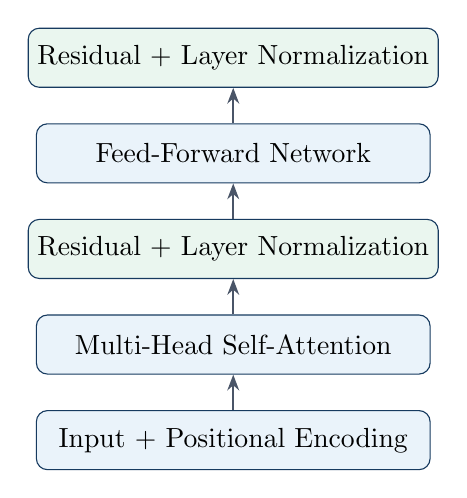
\begin{tikzpicture}[
  block/.style={draw=navy,rounded corners,fill=lightblue,minimum width=5.0cm,minimum height=0.75cm,align=center},
  arr/.style={-{Stealth[length=2mm]},thick,color=darkgray}
]
  \node[block] (x) {Input + Positional Encoding};
  \node[block,above=0.45cm of x] (a) {Multi-Head Self-Attention};
  \node[block,above=0.45cm of a,fill=lightgreen] (n1) {Residual + Layer Normalization};
  \node[block,above=0.45cm of n1] (f) {Feed-Forward Network};
  \node[block,above=0.45cm of f,fill=lightgreen] (n2) {Residual + Layer Normalization};
  \draw[arr] (x)--(a); \draw[arr] (a)--(n1); \draw[arr] (n1)--(f); \draw[arr] (f)--(n2);
\end{tikzpicture}
\end{center}

\subsection*{1. Residual Connection and Layer Normalization}

A residual connection forms

\[
r=x+\operatorname{Sublayer}(x).
\]

Layer normalization is

\[
\boxed{
\operatorname{LN}(r_i)
=\gamma\frac{r_i-\mu}{\sqrt{\sigma^2+\epsilon}}+\beta
}.
\]

\textbf{Worked example: residual plus normalization.}

Let

\[
x=(1,2),
\qquad
z_{\mathrm{att}}=(0.4,0.6).
\]

The residual vector is

\[
r=x+z_{\mathrm{att}}=(1.4,2.6).
\]

Its mean is

\[
\mu=\frac{1.4+2.6}{2}=2.
\]

Its variance is

\[
\sigma^2=\frac{(1.4-2)^2+(2.6-2)^2}{2}=0.36.
\]

With $\gamma=1$, $\beta=0$, and negligible $\epsilon$,

\[
\operatorname{LN}(r)
=\left(\frac{-0.6}{0.6},\frac{0.6}{0.6}\right)
=(-1,1).
\]

\[
\boxed{\operatorname{LN}(x+z_{\mathrm{att}})=(-1,1).}
\]

\subsection*{2. Position-Wise Feed-Forward Network}

The Transformer feed-forward network is

\[
\boxed{
\operatorname{FFN}(x)
=\operatorname{ReLU}(xW_1+b_1)W_2+b_2
}.
\]

It is applied independently to every sequence position.

\textbf{Worked example: one token through an FFN.}

Let

\[
x=\begin{bmatrix}1&-1\end{bmatrix},
\quad
W_1=
\begin{bmatrix}
1&2\\
-1&1
\end{bmatrix},
\quad b_1=(0,0).
\]

Then

\[
xW_1=(2,1).
\]

After ReLU,

\[
u=\operatorname{ReLU}(2,1)=(2,1).
\]

Let

\[
W_2=\begin{bmatrix}0.5\\1\end{bmatrix},
\qquad b_2=0.
\]

Therefore,

\[
\operatorname{FFN}(x)=2(0.5)+1(1)=2.
\]

\[
\boxed{\operatorname{FFN}(x)=2.}
\]

\subsection*{3. Decoder Probability}

The Transformer decoder models

\[
\boxed{
P(y\mid x)=\prod_tP(y_t\mid y_{<t},x)
}.
\]

\textbf{Worked example: softmax output and cross-entropy.}

Suppose the vocabulary logits at one decoding step are

\[
z=(2.0,1.0,0.0).
\]

Softmax gives

\[
p_i=\frac{e^{z_i}}{e^2+e^1+e^0}.
\]

Since

\[
e^2+e^1+e^0=7.389+2.718+1=11.107,
\]

we obtain

\[
p=(0.665,0.245,0.090).
\]

If the first token is correct, the cross-entropy loss is

\[
L=-\log(0.665)=0.408.
\]

\[
\boxed{p=(0.665,0.245,0.090),\qquad L=0.408.}
\]

% ============================================================
\section*{IX. RNNs versus Transformers}
% ============================================================

\begin{center}
\begin{tabularx}{0.97\textwidth}{>{\bfseries}p{3.0cm}XX}
\toprule
Property&RNN, LSTM, or GRU&Transformer\\ \midrule
Processing&Sequential recurrence&Parallel across positions during training\\
Memory&Hidden or cell state&Attention-based representation\\
Long dependencies&May be difficult&Direct attention path\\
Streaming&Natural&Requires causal or chunked design\\
Long-sequence cost&Sequential in $T$&Standard attention is quadratic in $T$\\
Small data&Often effective&Often benefits from pretraining\\ \bottomrule
\end{tabularx}
\end{center}

\subsection*{Worked Example: Computational Scaling}

For an approximate comparison, recurrent hidden-state computation contains a term proportional to

\[
T d^2,
\]

while the attention-score computation contains a term proportional to

\[
T^2d.
\]

Let $T=100$ and $d=64$.

RNN-style recurrent work is approximately

\[
100(64^2)=409{,}600
\]

multiplication units, performed sequentially across $100$ steps.

Attention-score work is approximately

\[
100^2(64)=640{,}000
\]

multiplication units, but the token-pair computations can be parallelized.

For $T=1000$,

\[
T^2d=1000^2(64)=64{,}000{,}000,
\]

showing why standard attention becomes expensive for very long sequences.

\begin{center}
\begin{tabular}{c|c|c}
\toprule
Length $T$&Recurrent term $Td^2$&Attention-score term $T^2d$\\ \midrule
$100$&$409{,}600$&$640{,}000$\\
$1000$&$4{,}096{,}000$&$64{,}000{,}000$\\ \bottomrule
\end{tabular}
\end{center}

\keybox{lightorange}{\textbf{Model-selection principle.} Transformers provide short attention paths and parallel training, but recurrent models remain useful for compact causal or streaming systems. The correct choice depends on data size, sequence length, latency, causality, hardware, and pretraining availability.}

% ============================================================
\section*{X. Applications and Model Selection}
% ============================================================

\begin{center}
\begin{tabularx}{0.98\textwidth}{>{\bfseries}p{3.0cm}XX}
\toprule
Domain&Applications&Suitable models\\ \midrule
Natural language&Sentiment, translation, summarization, QA&BiRNN, LSTM, Transformer\\
Speech&Recognition, synthesis, translation&LSTM, GRU, Transformer\\
Time series&Forecasting, monitoring, anomaly detection&RNN, LSTM, Transformer\\
Recommendation&Next-item and click prediction&GRU, sequential Transformer\\
Computer vision&Classification and detection&Vision Transformer\\
Healthcare&Patient-event prediction&LSTM, Transformer\\
Multimodal AI&Text-image and audio-text modeling&Transformer architectures\\ \bottomrule
\end{tabularx}
\end{center}

\subsection*{Worked Example: Choosing a Model}

Suppose three applications have the following requirements.

\begin{center}
\begin{tabularx}{0.97\textwidth}{>{\bfseries}p{3.0cm}XX}
\toprule
Application&Important conditions&Recommended starting model\\ \midrule
Live sensor prediction&One sample at a time, strict causality, limited hardware&GRU\\
Machine translation&Long context, large parallel hardware, pretrained models&Transformer\\
Small medical sequence set&Limited labeled data, moderate sequence length&Regularized LSTM or GRU\\ \bottomrule
\end{tabularx}
\end{center}

The recommendation follows the constraints, not a claim that one architecture is universally best.

% ============================================================
\section*{XI. Practice Problems}
% ============================================================

\begin{enumerate}
  \item For $h_t=\tanh(0.4x_t+0.5h_{t-1})$, calculate $h_1$ when $x_1=2$ and $h_0=0$.
  \item A recurrent derivative factor is $0.7$. Calculate its magnitude after eight steps.
  \item In an LSTM, $f_t=0.8$, $c_{t-1}=0.5$, $i_t=0.4$, and $\tilde c_t=0.6$. Calculate $c_t$.
  \item In a GRU, $z_t=0.25$, $h_{t-1}=0.8$, and $\tilde h_t=0.2$. Calculate $h_t$.
  \item A three-token target has conditional probabilities $0.9$, $0.8$, and $0.7$. Calculate its sequence probability.
  \item Convert attention scores $(0,1)$ into softmax weights.
  \item For $q=(1,0)$ and $k=(2,3)$, calculate the dot-product attention score.
  \item For sequence length $T=50$, how many entries are in the full $T\times T$ attention-score matrix?
  \item Compute $PE(0,0)$ and $PE(0,1)$ for sinusoidal positional encoding.
  \item A model gives probability $0.8$ to the correct token. Calculate its cross-entropy loss.
\end{enumerate}

\textbf{Answer check.}

\begin{enumerate}
  \item $h_1=\tanh(0.8)\approx0.6640$.
  \item $(0.7)^8\approx0.05765$.
  \item $c_t=0.8(0.5)+0.4(0.6)=0.64$.
  \item $h_t=(1-0.25)(0.8)+0.25(0.2)=0.65$.
  \item $0.9(0.8)(0.7)=0.504$.
  \item $\softmax(0,1)=(1/(1+e),e/(1+e))\approx(0.269,0.731)$.
  \item $q^\top k=1(2)+0(3)=2$.
  \item $50^2=2500$ entries.
  \item $PE(0,0)=\sin(0)=0$ and $PE(0,1)=\cos(0)=1$.
  \item $L=-\log(0.8)\approx0.223$.
\end{enumerate}

% ============================================================
\section*{XII. Key Takeaways}
% ============================================================

\begin{enumerate}
  \item RNNs share recurrent parameters and summarize earlier information in hidden states.
  \item BPTT creates products of derivatives, which can vanish or explode across long sequences.
  \item LSTM and GRU gates regulate forgetting, writing, and exposing recurrent information.
  \item Basic Seq2Seq compresses a source sequence into a context vector and factorizes target probability autoregressively.
  \item Attention constructs a different weighted context for each query.
  \item Transformer attention uses query, key, and value matrices with scaled dot products.
  \item Causal masks prevent a decoder from using future target tokens.
  \item Multi-head attention learns several interaction patterns, while positional encoding supplies order information.
  \item Residual connections, layer normalization, and feed-forward networks complete the Transformer layer.
  \item Architecture selection should consider sequence length, causality, latency, data volume, hardware, and pretraining.
\end{enumerate}

% ============================================================
\section*{References}
% ============================================================

\begin{enumerate}[label={[\arabic*]}]
  \item S. Hochreiter and J. Schmidhuber, ``Long Short-Term Memory,'' \textit{Neural Computation}, vol. 9, no. 8, 1997.
  \item M. Schuster and K. K. Paliwal, ``Bidirectional Recurrent Neural Networks,'' \textit{IEEE Transactions on Signal Processing}, vol. 45, no. 11, 1997.
  \item I. Sutskever, O. Vinyals, and Q. V. Le, ``Sequence to Sequence Learning with Neural Networks,'' \textit{NeurIPS}, 2014.
  \item D. Bahdanau, K. Cho, and Y. Bengio, ``Neural Machine Translation by Jointly Learning to Align and Translate,'' \textit{ICLR}, 2015.
  \item A. Vaswani et al., ``Attention Is All You Need,'' \textit{NeurIPS}, 2017.
  \item A. Zhang et al., \textit{Dive into Deep Learning}, Cambridge University Press, 2023.
\end{enumerate}

\end{document}
